\documentclass{article}
\usepackage{graphicx} % Required for including images
\usepackage{booktabs} % For professional looking tables
\usepackage{makecell} % For line breaks in table cells
\usepackage{amsmath}  % For math symbols if needed
\usepackage{parskip}  % Add space between paragraphs
\setlength{\parindent}{0pt} % Remove paragraph indentation
\usepackage[margin=1in]{geometry} % Set margins to 1 inch
\usepackage{tikz}
\usepackage{pgfplots}
\pgfplotsset{compat=1.17}
\usepackage{standalone}
\usetikzlibrary{positioning,arrows.meta,calc,decorations.pathmorphing,fit,shapes.geometric}

\title{Quantum Eraser Experiment Results: Visibilities and Graphs (2025-06-02)}
\author{Group 13} % Assuming the same group as lab-6-entangled.tex
\date{\today}

\begin{document}
\pagestyle{empty} % No page numbers for a single page doc

%% Custom style for quantum optics
\tikzset{
    >={Straight Barb[width=3pt,length=3pt]},  % Narrower default arrow
    photon/.style={thick, red},
    detector/.style={
        draw=black, 
        semicircle,
        minimum width=0.6cm,
        minimum height=0.6cm,
        inner sep=0pt,
        outer sep=0pt,
        fill=yellow!10, 
        text=black
    },
    hwp/.style={draw, rectangle, minimum width=0.25cm, minimum height=0.75cm, fill=blue!10, thick},
    lp/.style={draw, rectangle, minimum width=0.25cm, minimum height=0.75cm, fill=gray!10, thick},
    box/.style={draw, rectangle, rounded corners, inner sep=6pt},
    beamsplitter/.style={
        minimum width=0.5cm,
        minimum height=0.5cm,
        path picture={
            \draw[very thick,dashed] (path picture bounding box.north east) -- (path picture bounding box.south west);
        }
    },
    pbs/.style={draw, rectangle, minimum width=1cm, minimum height=1cm, fill=gray!20, thick},
    mirror/.style={
        minimum width=0.5cm,
        minimum height=0.5cm,
        path picture={
            \draw[very thick] (path picture bounding box.north east) -- (path picture bounding box.south west);
        }
    },
    stage/.style={
        minimum width=0.5cm,
        minimum height=0.5cm,
        path picture={
            \draw[<->,very thick] (path picture bounding box.north west) -- (path picture bounding box.south east);
        }
    },
}

\begin{figure}[htbp]
\centering
\resizebox{\linewidth}{!}{%
\begin{tikzpicture}[scale=1.8]
    
    % Source
  \node[draw, circle, minimum size=0.5cm] (S) at (0,0) {\small S};

  \node[draw, rectangle, minimum width=0.25cm, minimum height=0.75cm, fill=red!10, thick,rotate=0,right=0.75cm of S] (FW) {};
  \node[below=0.25cm of FW] () {\small Filter Wheel};
  
  \node[hwp,rotate=0,right=3.25cm of S] (HWP) {};
  \node[below=0.25cm of HWP] () {\small HWP$_p(22.5^\circ)$};

  
    \node[draw, rectangle, minimum size=0.5cm, right=5cm of S] (BIBO) at (0,0) {\small BiBO};
    % Idler arm: Mach-Zehnder interferometer (MZI)
    \node[beamsplitter, right=1.5cm of BIBO] (BS1) {};
    \node[below=0.4cm of BS1] () {\small BS$_1$};

    \node[mirror, above=2.5cm of BS1] (M1) {};
    \node[mirror, right=2.5cm of BS1] (M2) {};
    \node[stage] at ($(M2)+(0.2cm,-0.2cm)$) (STAGE) {};
    \node at ($(STAGE)+(0.15cm,0.15cm)$) {$\varphi$};
    \node[right=.4cm of STAGE,align=left] {\small Piezo-controlled\\stage};


    \node[beamsplitter, right=2.5cm of M1] (BS2) {};
    \node at ($(BS2)-(0.3,0.3)$) {\small BS$_2$};

    \node[detector,rotate=270] (DI) at ($(BS2.east)+(1.5cm,0)$) {\rotatebox{90}{\small $D_i$}};

    % Signal arm: LP with detector
    \node[lp,rotate=270] at ($(BIBO)+(0,1.75cm)$) (LPs) {};
    \node[left=0.5cm of LPs] () {\small LP$_s(\theta_s)$};
    \node[detector,rotate=0, above=4cm of BIBO] (DS) {\small $D_s$};

    \node[lp,rotate=0,right=1cm of BS2] (MZI_LP) {};
    \node[below=0.1cm of MZI_LP] () {\small LP$_i(90^\circ)$};

     % For Lab 6
     \node[hwp,rotate=0,right=1.25cm of M1] (MZI_HWP) {};
     \node[above=0.1cm of MZI_HWP] () {\small HWP$_t(45^\circ)$};
     \node[hwp,rotate=0,right=1.25cm of BS1] (MZI_HWP2) {};
     \node[below=0.25cm of MZI_HWP2] () {\small HWP$_b(0^\circ)$};

    % Pump and photon paths
    \draw[->, thick, red] (S) -- (BIBO);

    % Signal (upper) photon
    \draw[->, thick, red] (BIBO) -- (DS);

    % Idler photon through the MZI
    \draw[-, thick, red] (BIBO) -- (BS1.center);
    \draw[-, thick, red] (BS1.center) -- (M1.center);
    \draw[-, thick, red] (BS1.center) -- (M2.center);
    \draw[-, thick, red] (M1.center) -- (BS2.center);
    \draw[->, thick, red] (M2.center) -- ($(BS2.north) + (0,.1cm)$);
    \draw[-, thick, red] (BS2.center) -- (BS2.center);
    \draw[->, thick, red] (BS2.center) -- (DI);
    
    % Coincidence Counter and connecting dashed lines
    \node[draw, rectangle] (CC) at ($(DI |- DS)$) {\small CC};
    \draw[-, dashed] (DI.west) -- (CC.south);
    \draw[-, dashed] (DS.east) -- (CC.west);

    % These overwrite the laser lines
    \node[lp,rotate=270,fill=gray!50,minimum height=1.5cm] at ($(BS1)+(-0.2,0.6cm)$) (SHUTTER) {};
    \node[align=right] at ($(SHUTTER)+(-0.4,0.35)$) {\small Shutter\\(retractable)};

  \node[draw, rectangle, minimum width=0.25cm, minimum height=1.5cm, fill=gray!50, thick,rotate=0] at ($(S)+(1.35cm,0.2)$) (PM) {};
  \node[above=0.25cm of PM,align=center] () {\small Power meter\\(retractable)};



\end{tikzpicture}
}% end resizebox
\caption{
Entangled pair quantum eraser experiment, where the signal photon's
polarization carries ``which-way'' information
about the idler's path through the MZI.
Uses the unchanged Lab 6 apparatus with settings:
1. Set the pump HWP$_p$ to $45^\circ$ to generate $|\Phi^+\rangle$ entangled pairs;
2. Vary the signal LP$_s$ angle $\theta_s$ to control the eraser.
Setting $\theta_s = 45^\circ$ erases the ``which-way'' information from the signal,
restoring self-interference of the idler in the MZI.
The idler does not self-interfere 
for $\theta_s \in \{0^\circ, 90^\circ\}$, as the which-way info remains on the signal.
\label{fig:apparatus}
}
\end{figure}


% The visibility values V_ON and V_OFF below are placeholders.
% Please replace them with the actual values obtained by running the coincidences.py script.
% The script will print lines like:
% Coincidence Visibility (eraser-on): X.XXX
% Coincidence Visibility (eraser-off): Y.YYY
\begin{table}[h!]
\centering
\begin{tabular}{lcc}
\toprule
Condition & \makecell{Signal \\ LP angle} & \makecell{Idler self-interference \\ visibility (V)} \\
\midrule
Eraser On          & $45^\circ$  & 0.577 \\
Eraser Off         & $0^\circ$ & 0.121 \\
Signal Blocked     & Blocked & 0.023 \\
\bottomrule
\end{tabular}
\caption{
  Observed visibilities for idler self-interference in the MZI,
  when erasing which-way information from the signal photon (or not)
  in the entangled quantum eraser experiment.}
\end{table}

\begin{figure}[h!]
\centering
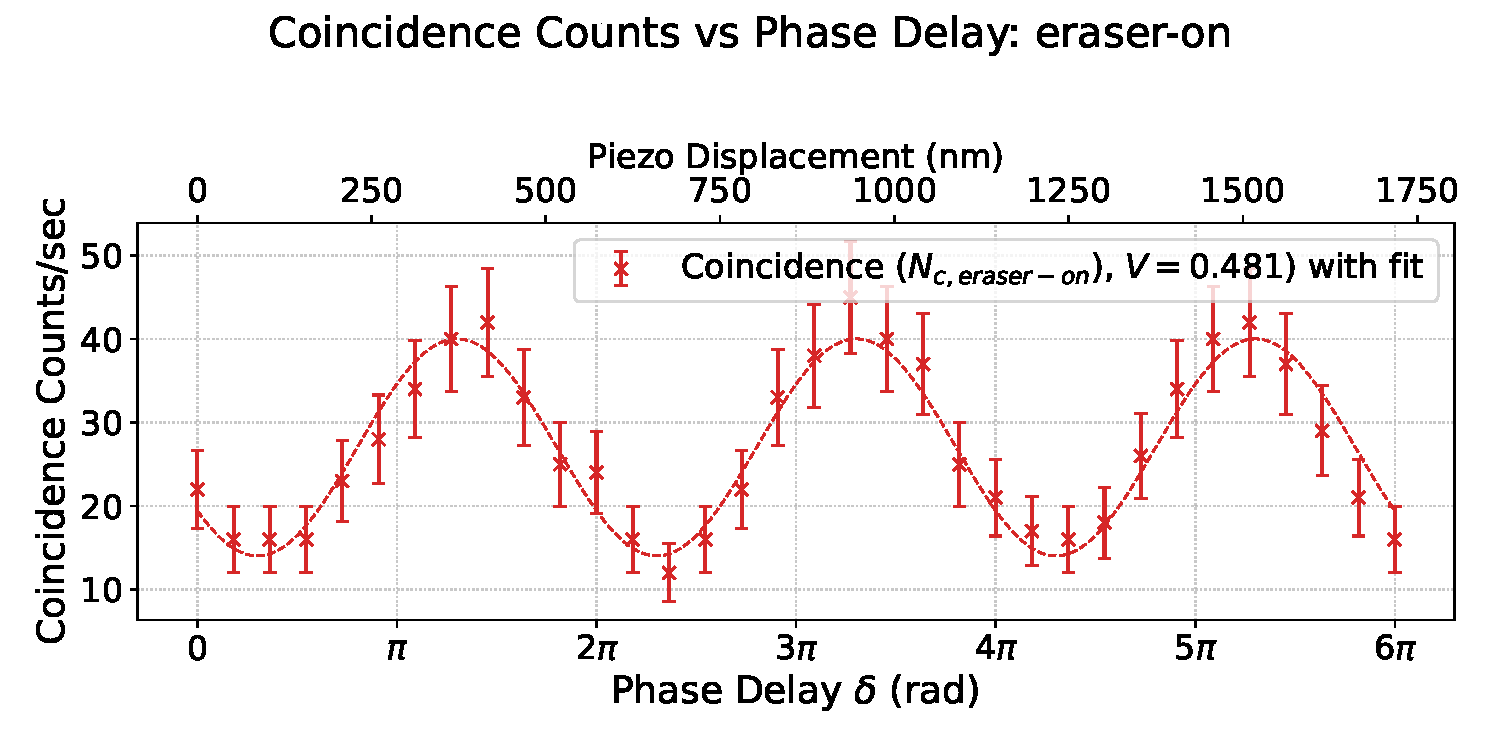
\includegraphics[width=0.6\textwidth]{coincidence_counts_eraser_on.pdf}
\caption{
  Erasing which-way info from the signals
  produced high visibility ($V=0.577$) idler self-interference.
}
\end{figure}


\begin{figure}[h!]
\centering
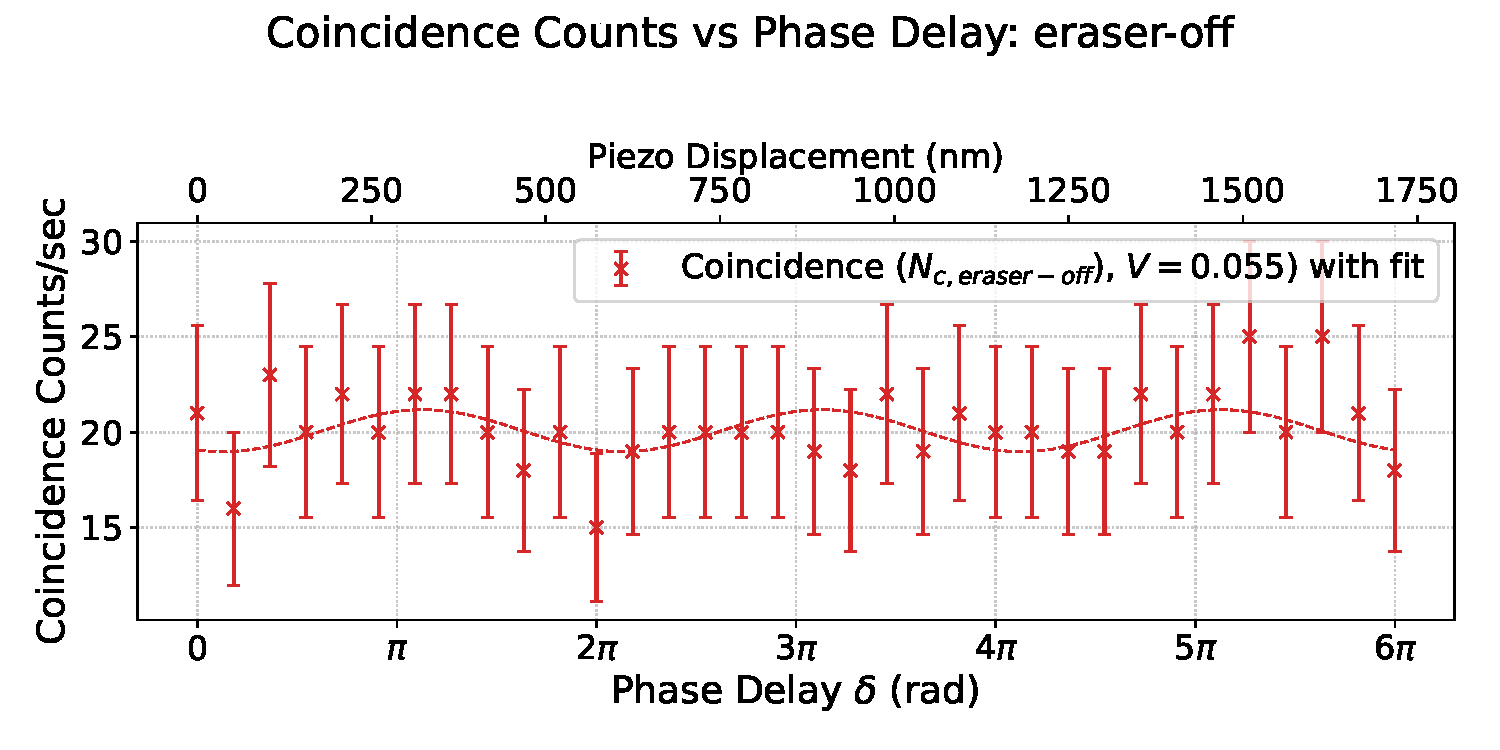
\includegraphics[width=0.6\textwidth]{coincidence_counts_eraser_off.pdf}
\caption{
  Not erasing which-way information from the signal photons
  prevented self-interference of the idlers in the MZI,
  resulting in low visibility ($V=0.121$).
  Coincidence counts vs Phase Delay with the eraser off.
}
\end{figure}

\begin{figure}[h!]
\centering
\includegraphics[width=0.6\textwidth]{coincidence_counts_signal_blocked.pdf}
\caption{
  With the signal beam completely blocked, no which-way information is available,
  but the very low visibility ($V=0.023$) indicates minimal interference due to
  lack of entanglement correlation. Coincidence counts vs Phase Delay with signal blocked.
}
\end{figure}

\end{document}
